\documentclass{article}
\usepackage[T1]{fontenc}
\usepackage{tgadventor}
\usepackage{geometry}
\usepackage{titling}
\usepackage{polski}
\usepackage{graphicx}
\usepackage{float}
\usepackage{indentfirst}

\renewcommand{\familydefault}{\sfdefault}

\geometry{
    top = 15mm,
    left = 25mm,
    right = 25mm,
    bottom = 25mm,
}

\begin{document}
    \begin{titlepage}
        \centering
        {\Huge\bfseries Autonomiczny robot społeczny ,,Rysiek''\par}
        
\includegraphics[width=0.5\textwidth]{figures/konar.png}\par
        {\huge Koło Naukowe Robotyków\\,,KoNaR''\par}
        {\par}\vspace{1cm}
        {\large Krzysztof Andrzejewski\par}
        {\large Wojciech Bohdan\par}
        {\large Krzysztof Kowaczek\par}
        {\large Tomasz Lubelski\par}
        {\large Michał Mastej\par}
        {\large Eryk Możdżeń\par}
        {\large Dominik Pluta\par}
        {\large Kamil Winnicki\par}
    \end{titlepage}

    \section{O projekcie}
        \subsection*{Motywacja}
            Wzrasta potrzeba technologii, które łączą funkcjonalność z empatyczną interakcją - zwłaszcza w~kontekście
            społeczeństw starzejących się, rosnącej samotności wśród młodych oraz sektorach usługowych (edukacja, opieka, rozrywka, handel).
            Rynek poszukuje rozwiązań, które nie tylko wykonują zadania, ale także budują emocjonalne więzi, redukują stres lub wspierają codzienne mikro-potrzeby
            (np. przypomnienie o lekach, inicjowanie kontaktu).
            Dodatkowo, rośnie popyt na przyjazne roboty edukacyjne dla dzieci, które uczą przez zabawę,
            oraz na automatyzację usług z elementami „osobowości” (np. hostele w gastronomii).

        \subsection*{Założenia projektowe}
            \begin{itemize}
                \item inicjowanie oraz potrzymywanie interrakcji z człowiekiem,
                \item komunikacja za pomocą kolorowych świateł i ruchów,
                \item możliwość implementacji różnych scenariuszy użycia,
                \item przyjazny \textit{design} zwierzęcia.
            \end{itemize}

        \subsection*{Cel}
            Stworzyć robota, który nie jest „narzędziem”, lecz partnerem w codziennych wyzwaniach -- od
            przpomnieniu o szklance wody, dawce leku lub zdrowej przkąsce po rozbawienie gestem.

    \section{Budowa mechaniczna}
        Realizując założenia projektowe zdecydowano się na sylwetkę rysia, głównie z powodu symptycznego usposobienia.
        Pełna konstrukcja została przedstawiona na rys. \ref{full_opisy}.
        \begin{figure}[p]
            \centering
            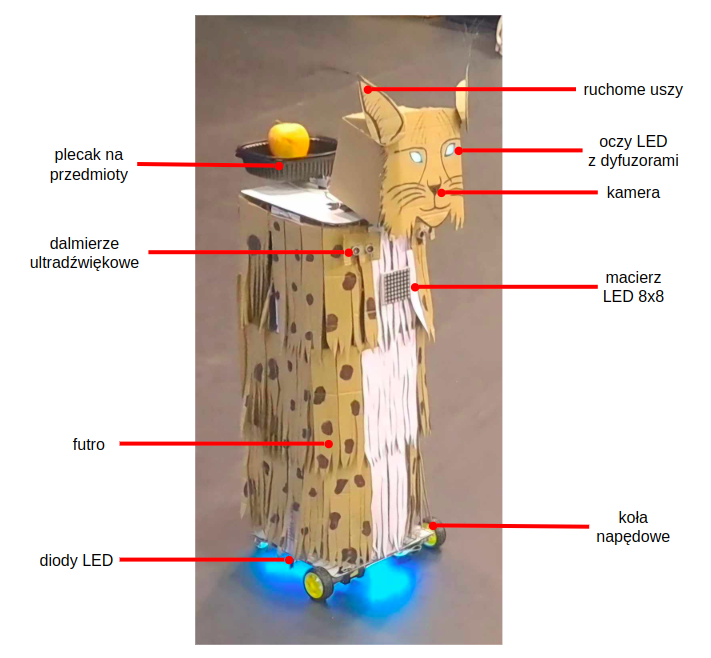
\includegraphics[width=0.75\textwidth]{figures/full_opisy.png}
            \caption{Widok robota z zewnątrz}
            \label{full_opisy}
        \end{figure}
        Robot składa się z:
        \begin{itemize}
            \item smukłej ramy nośnej wraz z silnikami napędowymi (rys. \ref{frame_opisy}),
            \item pokrycia wierzchniego ze spreparowanego karonu imitującego futro,
            \item animatronicznej głowy,
            \item pojemnika/plecaka na produkty zawieszonego na czujniku tensometrycznym,
        \end{itemize}
        \begin{figure}[p]
            \centering
            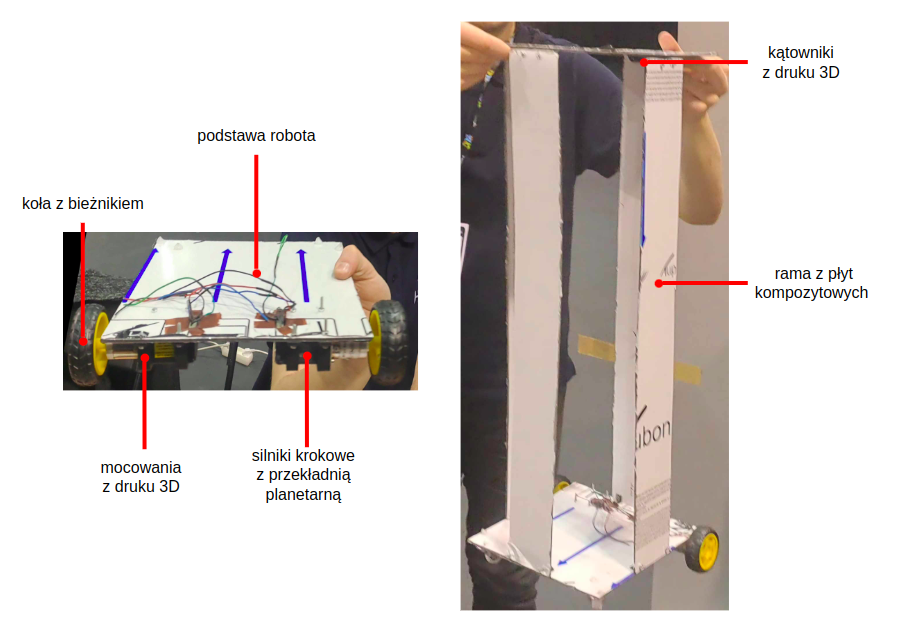
\includegraphics[width=0.85\textwidth]{figures/frame_opisy.png}
            \caption{Rama robota}
            \label{frame_opisy}
        \end{figure}

    \section{Układy elektroniki}
        Elektornika robota została wykonana ręcznie na podstawie płytki rozwojowej \textit{Nucleo} oraz płytki prototypowej.
        Uproszczony schemat połączeń przedstawia rys. \ref{elektronika_schemat}.
        \begin{figure}[p]
            \centering
            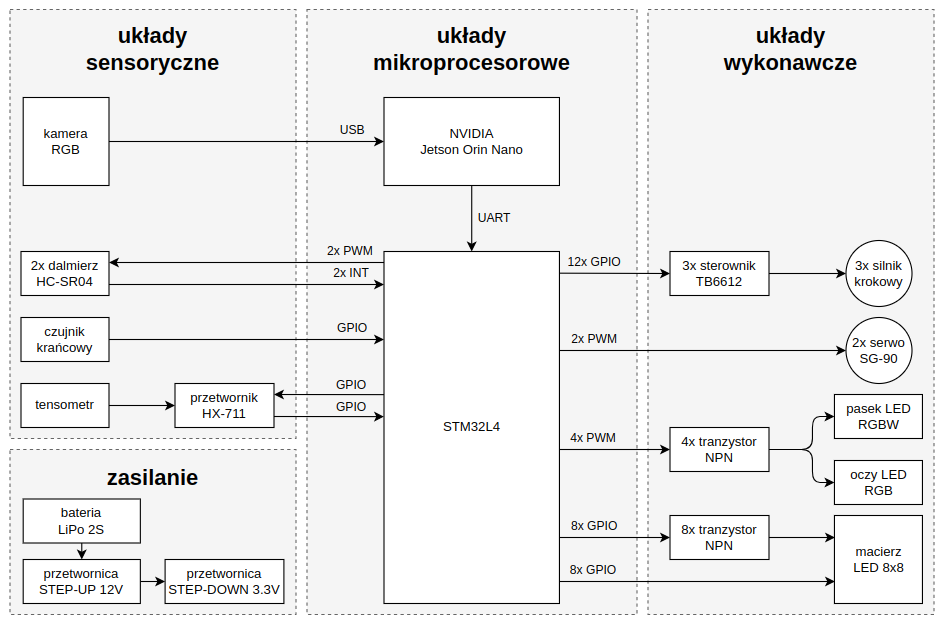
\includegraphics[width=\textwidth]{figures/elektronika_schemat.png}
            \caption{Uproszczony schemat układów elektroniki robota}
            \label{elektronika_schemat}
        \end{figure}

    \pagebreak
    \section{Oprogramowanie mikrokontrolera}
        W roli jednostki sterującej niskopoziomowymi funkcjonalościami robota wybrano mikrokontroler STM32L476
        umieszczony na płytce rozwojowej \textit{Nucleo}. Mikrokontroler odpowiada za:
        \begin{itemize}
            \item odczyt czujników,
            \item steroanie pozycją i prędkością napędów,
            \item sterowanie kolorem diód w oczach i w podwoziu,
            \item wyświetlanie obrazów na macierzy LED,
            \item komunikacja z sterownikiem nadrzędnym.
        \end{itemize}

        \subsection*{Układy sensoryczne}
            Robot wykorzystuje czujniki ultradźwiękowe HC-SR04 do pomiaru odległości.
            Sygnał wyzwalający ejst generowany przez timer w trybie PWM,
            a czas powrotu echa jest mierzony za pomocą przerwań GPIO i timera.
            Belka tensometryczna z przetwornikiem HX-711 monitoruje obciążenie w plecaku przekształca surowe dane na wartość w kilogramach.
            Dodatkowo, czujnik krańcowy umożliwia wyzeroanie obrotu mechanizmu głowy aby umozliwić steroanie pozycją jej wychelnia.

        \subsection*{Układy wykonawcze}
            Silniki krokowe są kontrolowane przez sterowniki TB6612 - sekwencja kroków realizowana jest poprzez dynamiczne przełączanie stanów pinów GPIO.
            Prędkość regulowana jest programowym dzielnikiem opartym na timerze.
            Serwomechanizmy SG-90 oraz pasek LED RGBW sterowane są sygnałami PWM.
            Macierz LED 8x8 jest odświeżana w przerwaniu timera, wykorzystując multipleksowanie rzędów i kolumn.

        \subsection*{Komunikacja}
            Mikrokontroler odbiera komendy sterujące z sterownika wyższego poziomu NVIDIA Jetson Orin Nano
            przez magistralę szeregową UART z protokołem własnej implementacji.
            Ramka danych (rys. \ref{ramka_danych}) zawiera:
            \begin{figure}[p]
                \centering
                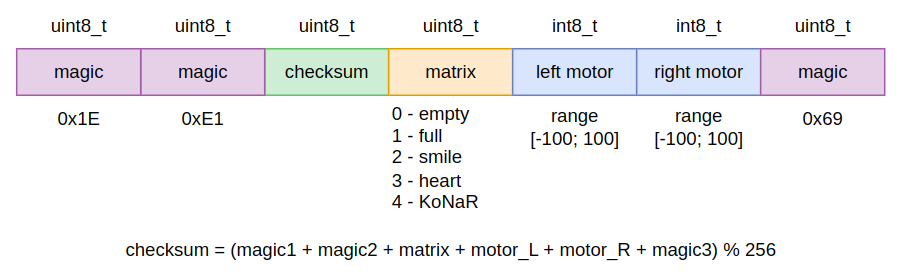
\includegraphics[width=\textwidth]{figures/ramka.png}
                \caption{Binarna ramka danych przychodząca ze sterownika nadrzędnego}
                \label{ramka_danych}
            \end{figure}
            \begin{itemize}
                \item bajty stałe do identyfikacji początku/końca ramki,
                \item jeden z predefiniowanych obrazów na matrycy LED,
                \item wartości prędkości silników,
                \item sumę kontrolną do analizy poprawności danych.
            \end{itemize}
            Dane odbierane są buforowo z użyciem DMA, a parser weryfikuje poprawność ramki przed aktualizacją stanu robota.

        \subsection*{Logika niskopoziomowa}
            STM32 działa jako niezależny system odpowiedzialny za bezpośrednie reakcje na zdarzenia fizyczne,
            nadpisując komendy z jednostki nadrzędnej (Jetson Orin Nano) w sytuacjach wymagających natychmiastowej reakcji.
            Gdy robot wykryje nagły ubytek masy w plecaku (np. gdy użytkownik zabierze smakołyk),
            mikrokontroler automatycznie zatrzymuje ruch silników, inicjuje animację „zadowolenia” na macierzy LED
            oraz wprowadza głowę i uszy w pozycję wyrażającą reakcję emocjonalną.

            Jednocześnie STM32 stale zarządza płynnymi ruchami głowy i mimiką LED, tworząc wrażenie „żywego” zachowania,
            nawet gdy wyższe warstwy oprogramowania skupiają się na zadaniach analitycznych.
            Ta warstwa zapewnia, że robot pozostaje responsywny i bezpieczny w bezpośrednich interakcjach z człowiekiem.

    \pagebreak
    \section{Oprogramowanie mikrokomputera}

\end{document}
